\subsection{Roulette Wheel und Stochastic Universal Sampling}
Bei dem von 'geatbx' angebotenem Verfahren 'selsus' handelt es sich um das
'Stochastic Universal Sampling'. Sowohl das 'selsus' wie auch das 'Roulette
Wheel'-Verfahren, dienen nach \cite{url:geatbx-documentation}
zur Auswahl der Paarungs-Populationen. Dabei erhalten die zu auszuwählenden
Individuen einen Bereich zugeteilt, der in seiner Größe relativ zum 
Fitnesswert und somit auch zur Auswahlwahrscheinlichkeit eines Individuums
steht. Beide Verfahren suchen nun per Zufall positionierter Zeiger, die
gewünschte Anzahl an Individuen aus. Der Unterschied zwischen dem 'Roulette-Wheel'
und dem 'selsus'-Verfahren besteht nun im Ziehungszeitpunkt. Während beim
'Roulette-Wheel'-Verfahren jedes Individuum in einem eigenen Durchlauf unabhängig
von den anderen gezogen wird, werden beim 'Stochastic Universal Sampling' alle
Individuen auf einmal gezogen. Durch diese Vorgehensweise sind die 
Auswahl-Wahrscheinlichkeiten voneinander, und damit von der jeweiligen Ziehung
abhängig, da es sich um Ziehen ohne Zurücklegen handelt.

Abbildung \ref{fig:RouletteSelsus} nach \cite{url:RouletteSelsus} verdeutlicht 
die oben beschriebenen Aspekte.
Es werden pro Selektionsverfahren je 4 Individuen, $Q_1$ bis $Q_4$ ausgewählt.
Beim 'Roulette-Wheel'-Verfahren finden dabei 4 Ziehungen statt, während beim
'selsus'-Verfahren 1 Ziehung durchgeführt wird.  

\begin{figure} 
  \centering
  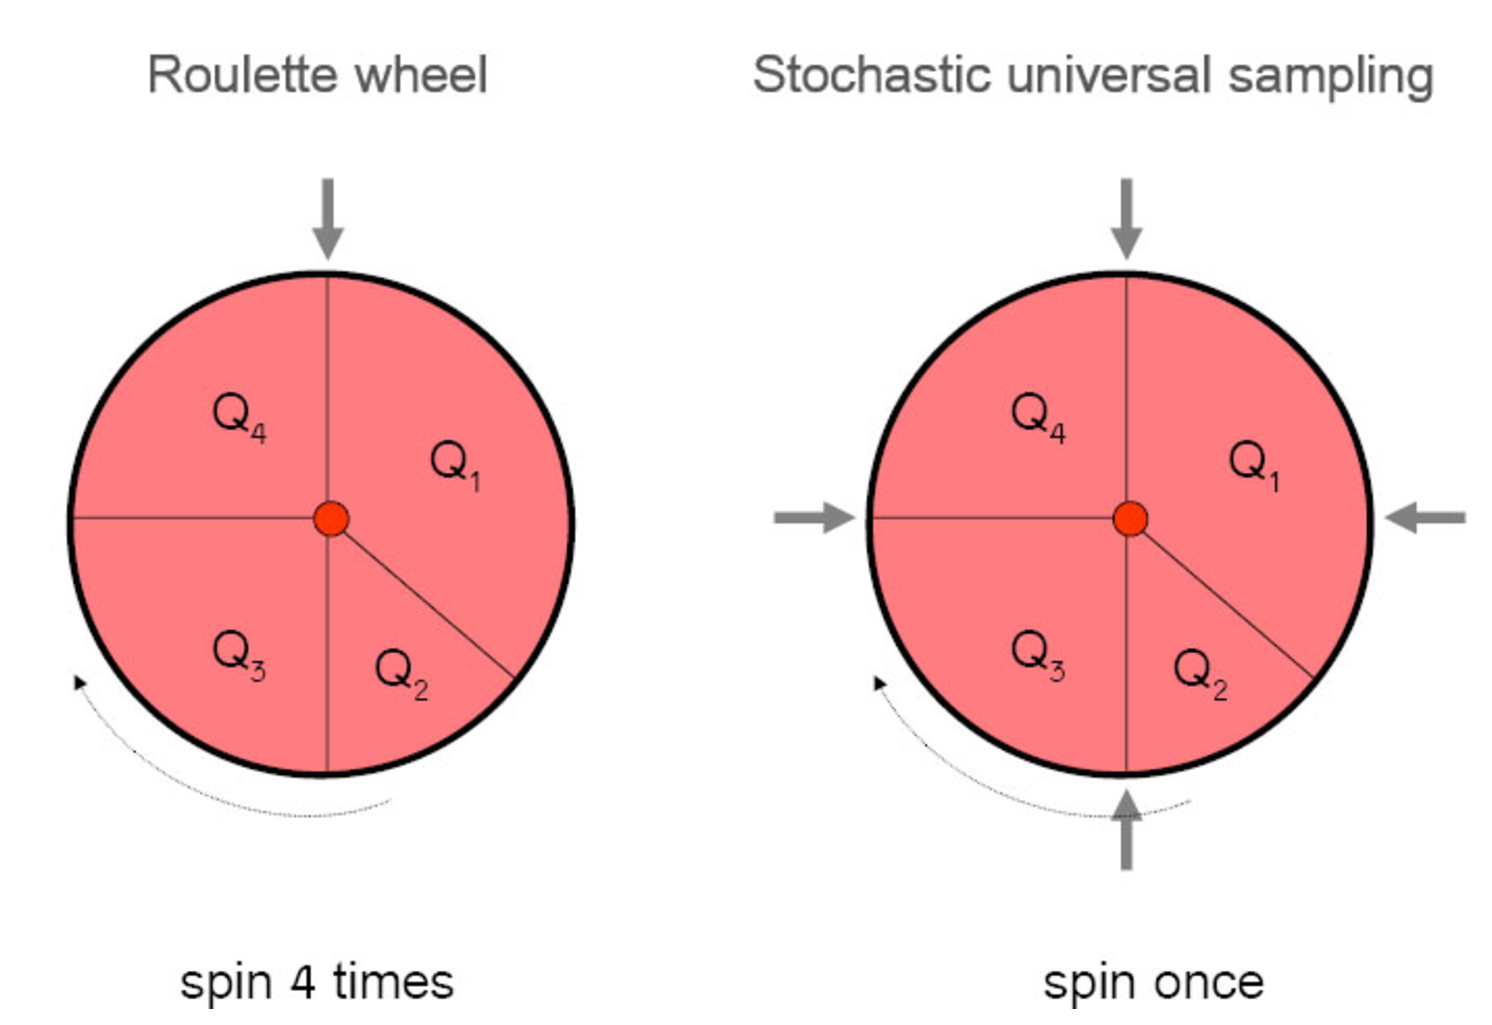
\includegraphics[width=0.6\textwidth]{../images/picRouletteSelsus}
  \caption{Selektionsverf. 'Roulette-Wheel' und 'Stochastic Universal Sampling'.}
  \label{fig:RouletteSelsus}
\end{figure}

Nachfolgende Abbildung nach \cite{url:geatbx-documentation} zeigt die von
\cite{url:geatbx-documentation} beschriebene Implementierung von 'selsus'.
Dabei werden die Zeiger, welche die Indiv. auswählen im gleichen Abstand
$1/n$ angeordnet sind. $n$ bezeichnet dabei die Anzahl der auszuwählenden
Individuen. Die Zufallszahl entscheidet nun über den Anfangspunkt der 
Zeigeranordnung, welche alle Individuen gleichzeitig wählt. In der Ziehung
des zeigten Beispiels nach \cite{url:geatbx-documentation}, ergeben sich 
hierdurch die Individuen 1, 2, 3, 4, 6, 8.
       
\begin{figure} 
  \centering
  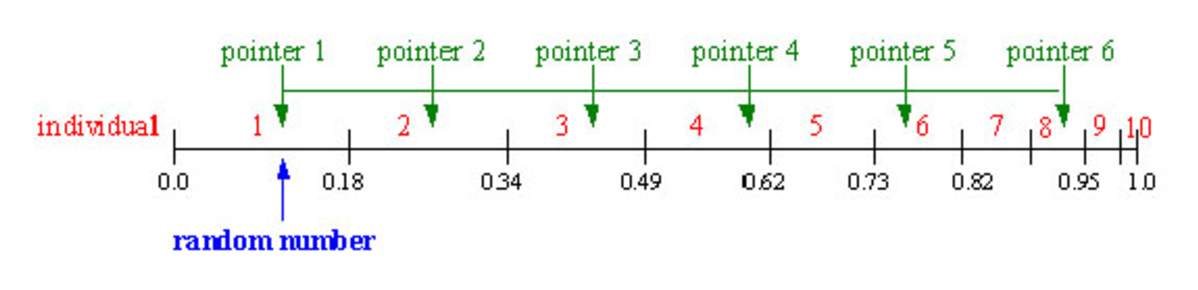
\includegraphics[width=0.8\textwidth]{../images/picSelsusAuswahl}
  \caption{Beispielziehung mit Hilfe des 'Stochastic Universal Sampling'.}
  \label{fig:SelsusAuswahl}
\end{figure}

\subsection{'Tournament'-Selektion}
Bei der 'Tournament'-Selektion lässt man nach \cite{url:geatbx-documentation}
zufällig ausgewählte Individuen gegeneinander antreten. Der jeweils fitteste
der 'Tournament'-Gruppe wird schließlich selektiert. Dieser Vorgang wird so
oft wiederholt, bis die gewünschte Anzahl an zu selektierenden Individuen
erreicht ist.

Folgende Abbildung nach \cite{url:RouletteSelsus} verdeutlicht dies.
Dabei werden aus einer Subpopulation zufällig drei Indiv. ausgewählt, die
gegeneinander antreten. Das Individuum mit dem höchsten Fitnesswert (hier $7$),
wird schließlich in den 'Mating-Pool' aufgenommen.

\begin{figure} 
  \centering
  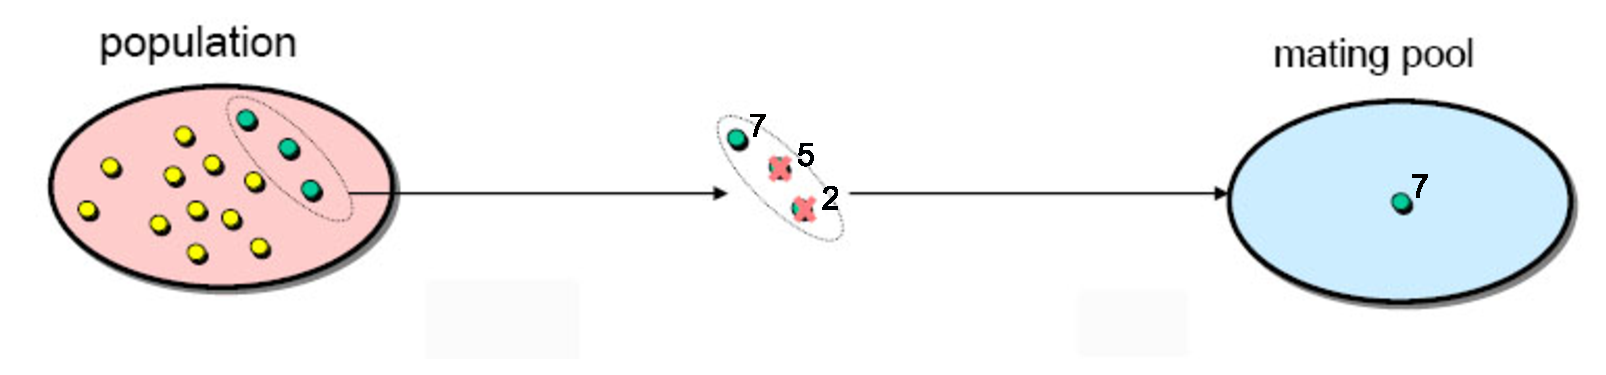
\includegraphics[width=0.8\textwidth]{../images/picTournamentAuswahl}
  \caption{Ziehung mit Hilfe der 'Tournament'-Selektion}
  \label{fig:TournamentAuswahl}
\end{figure}

\subsection{Testläufe mit variierenden Selektions-Methoden}
\label{subsec:TestlaufeSelektionsmethoden}
Für die Durchführung der Testreihen in Aufgabe d), wurde die in 
\ref{subsec:ArchitekturTestsystem} beschriebene Modifikation des
Testskriptes benutzt. 

\begin{description}
  \item[Selektions-Methoden:] selsus, selrws, seltour
\end{description}

Für jeden der 3 Selektionsarten wurden 20 Testläufe gefahren, womit 
sich eine Gesamtgröße von 60 Testläufen ergibt. Die in Aufgabe c) bereits durchgeführte
Testreihe von 12 Subpopulationen, 60 Individuen und der Selektionsart 'selsus',
wurde wiederholt. Die Ergebnisse ähneln dabei den in Tabelle 
\ref{tbl:aufgabeC-ergebnisse}
gezeigten Werten. So beträgt der Mittelwert aller wiederholten Testläufe
$2225.70$, während er in Aufgabe c) bei $2285.85$ lag. Vergleiche hierzu die
Ergebnisse aus Tabelle \ref{tbl:aufgabeD-ergebnisse}, der Zeile 1, mit den
Ergebnissen aus Tabelle \ref{tbl:aufgabeC-ergebnisse}, Testlauf Nr. 16.
Die vollständigen Testläufe, zu allen Selektionsarten, sind dem Anhang in Form
der entsprechenden Logging-Dateien zu entnehmen. 

\begin{table}
	\sffamily
	\centering
	\footnotesize
	\begin{tabularx}{\textwidth}{NXlllll}
		\toprule
		\multicolumn{1}{@{}N}{Selektion} &
		\multicolumn{1}{V{3.5em}@{}}{Subpop.} &
		\multicolumn{1}{V{3.5em}@{}}{Indiv.} &
		\multicolumn{1}{V{5em}@{}}{Mittelwert $\bar{x}$} &
		\multicolumn{1}{V{6.5em}@{}}{Standardabw. $\sigma_x$} &
		\multicolumn{1}{V{9em}@{}}{Minimalwert in Lauf $r$, Generation $g$} &
		\multicolumn{1}{V{9em}@{}}{Maximalwert in Lauf $r$, Generation $g$} \\
		\midrule\addlinespace
		
		selsus & 12 & 60 & 2225.70 & 119.76 & \textbf{2028}, $r = 1$, $g = 92$ & 2445, $r = 7$, $g = 100$ \\ \cmidrule(lr){1-7}
		selrws & 12 & 60 & 2234.45 & 113.72 & 2090, $r = 5$, $g = 99$ & 2479, $r = 18$, $g = 100$ \\ \cmidrule(lr){1-7}
		seltour & 12 & 60 & \textbf{2163.90} & 96.21 & 2036, $r = 1$, $g = 93$ & 2422, $r = 16$, $g = 94$ \\

		\addlinespace\bottomrule
		\end{tabularx}
	\caption{Ergebnisse aus 60 Testläufen, mit den Selektionsverfahren 'selsus', 'selrws' und 'seltour'.}
	\label{tbl:aufgabeD-ergebnisse}
\end{table}
 
\subsubsection{Interpretation der Ergebnisse}
Die Wiederholungstestläufe, die mit Hilfe der Selektionsart 'selsus' erzielt
wurden, ähneln  den Ergebnissen aus Kapitel \ref{subsec:TestlaeufePopulationsgroessen}.
Mit $2225.70$, konnte sogar ein leicht verbesserter Mittelwert erzielt werden. Allerdings
weichen dabei die einzelnen Werte mit einer Standardabweichung von $119.76$ km,
auch mehr vom Mittelwert ab, als in den Testläufen der Aufgabe c). Bei fest
vorgegebenen Parameterwerten von 12 Subpopulationen und 60 Individuen, liefert
das 'Roulette-Wheel'-Selektionsverfahren leicht schlechtere Ergebnisse als mit den
ersten 20 Testläufen des 'selsus'-Selektionsverfahrens. Das beste Ergebnis
lieferte die 'selsus'-Selektion mit einem minimalen Wert von 2028 Kilometern.
Im Mittel aller Werte lieferte jedoch die 'Tournament'-Selektion, mit $2163.90$ Kilometern
den besten Wert. Die einzelnen Werte zeigen dabei mit einer Standardabweichung von $96.21$ km,
eine verhältnismäßig geringe Streuung um den Mittelwert. Das schlechteste Ergebnis der
Selektionsart 'seltour', liegt mit $2422$ ebenfalls jeweils unter den Maximalwerten
der beiden ersten Selektionsarten, wie in Tabelle \ref{tbl:aufgabeD-ergebnisse}
gezeigt.
  
Somit konnte durch Ersetzen der Selektionsart 'selsus' durch das
'Roulette-Wheel'-Verfahren, keine signifikante Änderung der Ergebnisse erzielt
werden. Der Minimal- sowie der Mittelwert erreichten ein leicht schlechteres
Gesamtergebnis, welches keine genaueren Rückschlüsse zulässt. Durch Verwenden der 
'Tournament'-Selektionsart ergab sich optisch eine leichte Verbesserung des
Mittelwerts, welche jedoch prozententual ebenfalls nicht ins Gewicht fällt. 

Jedoch ergeben sich innerhalb des Verlaufs einer Testreihe gewisse Unterschiede.
Abbildung \ref{fig:aufgabeDMittelwerte} zeigt hierzu den Verlauf der kumulierten
Mittelwerte, für jeden der drei Testreihen.

\begin{figure} 
  \centering
  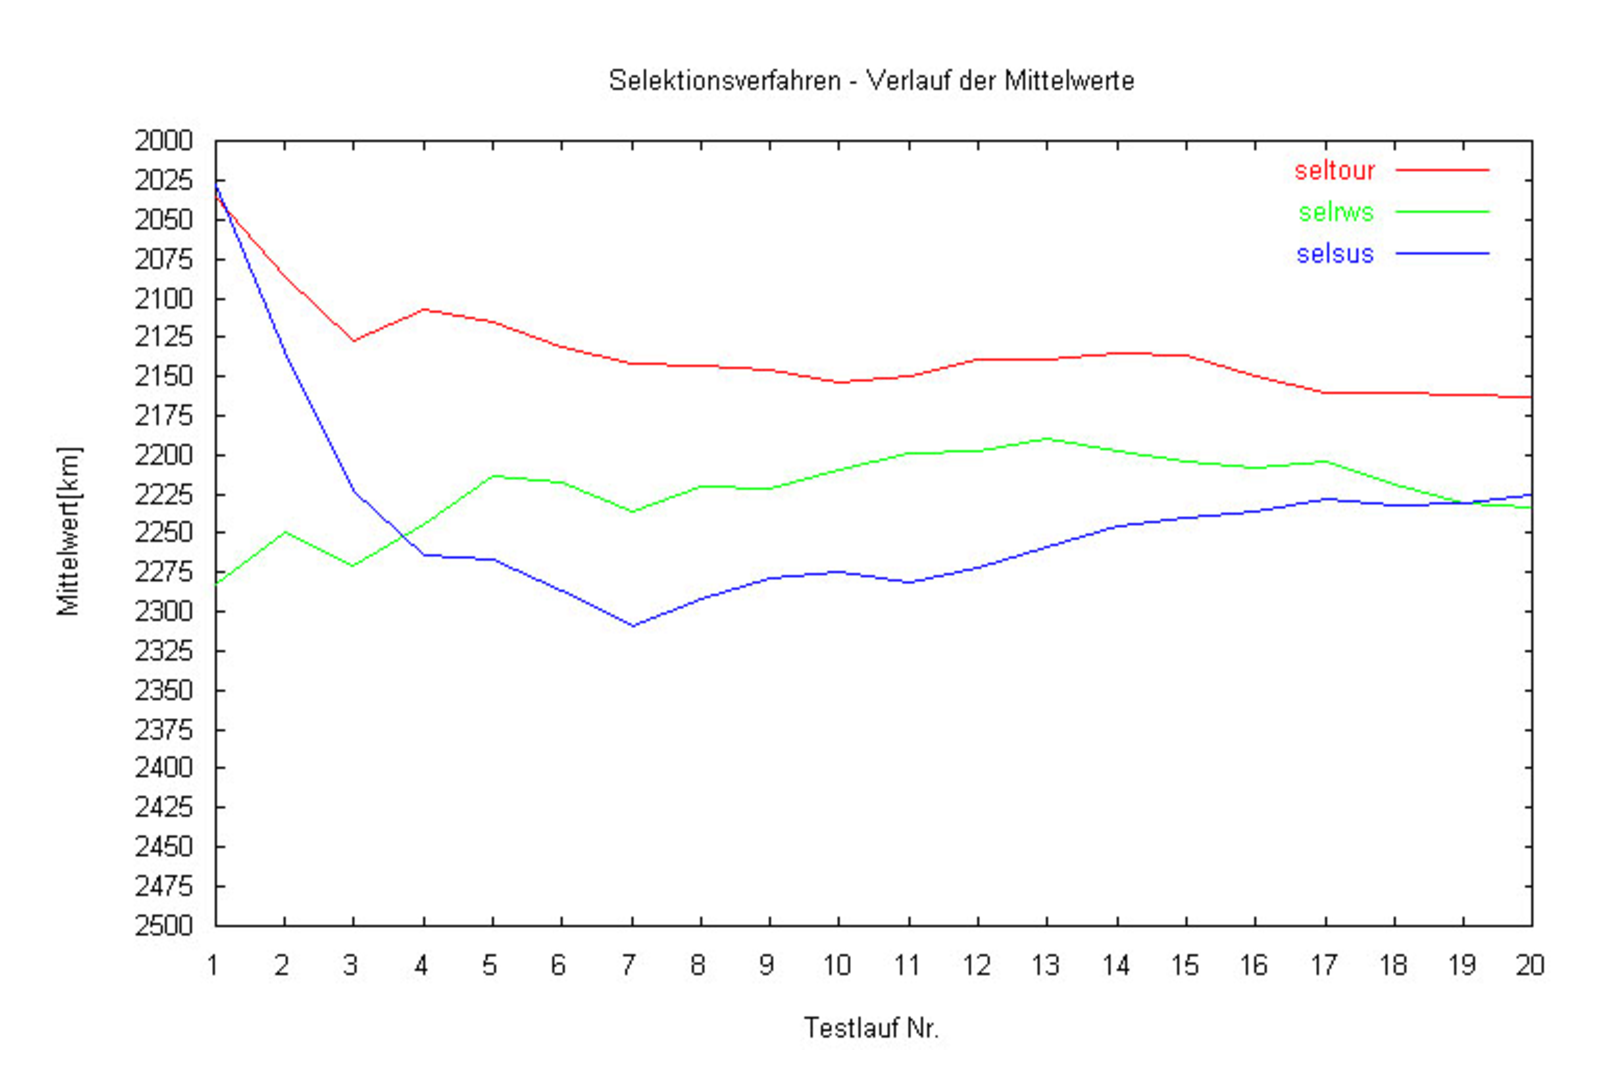
\includegraphics[width=1.0\textwidth]{../images/picMittelverlaufSelections}
  \caption{Verlauf der Mittelwerte der Selektionsarten 'selsus', 'selrws' und 'seltour'.}
  \label{fig:aufgabeDMittelwerte}
\end{figure}

Jedes der drei Verfahren zeigt eine Konvergenz der Mittelwerte gegen den Bereich 
$2150$ bis $2250$. Das 'selsus'-Verfahren erreicht früh seine besten Wert, fällt
dann aber steil ab und kovergiert die restlichen Läufe gegen den Konvergenzbereich.
Das Roulette-Wheel-Verfahren beginnt relativ schlecht und konvergiert schnell. Das
Tournament-Verfahren erreicht ebenfalls zu Beginn seinen besten Wert und konvergiert
auf etwas höherem Niveau als das 'selsus'-Verfahren gegen den Konvergenzbereich. 
